\documentclass[12pt, oneside]{book}
\usepackage[top=1in, bottom=1in, left=1.2in, right=1in, a4paper]{geometry}
\title{Graph Based Storage for Relational Databases}
\author{Adarsh Mohata, Ajith P S, Ashish Kedia, Sourabh Suman}

 \ifx\pdftexversion\undefined
 \usepackage[dvips]{graphicx}
 \else
 
 \usepackage[pdftex]{graphicx}
 \DeclareGraphicsRule{*}{mps}{*}{}
 \fi
\usepackage{url}
\usepackage{tabularx}
\usepackage{chapterbib}
\usepackage{hyperref}
\usepackage{lscape}
\usepackage{longtable}
\usepackage{float}
\usepackage{url}
\usepackage{amsmath}
\usepackage{multicol}
\usepackage{color}
\usepackage[utf8]{inputenc}
\usepackage{listings}
\usepackage{kbordermatrix}
\usepackage{fancyhdr}
\usepackage{caption}
\usepackage{chngcntr}
\usepackage{pdfpages}
\usepackage{amsmath}
\counterwithin{figure}{chapter}
\counterwithin{table}{chapter}
%\pagestyle{fancy}
\lhead{\leftmark}
\rhead{}
\cfoot{}
\rfoot{\thepage}
\raggedbottom
\renewcommand{\bibname}{References}
\newcommand{\project}{Graph Based Storage for Relational Databases}
\setcounter{secnumdepth}{4}
\setcounter{tocdepth}{4}

\definecolor{codegreen}{rgb}{0,0.6,0}
\definecolor{codegray}{rgb}{0.5,0.5,0.5}
\definecolor{codepurple}{rgb}{0.58,0,0.82}
\definecolor{backcolour}{rgb}{0.95,0.95,0.92}

\lstdefinestyle{mystyle}
{   language=bash,
    basicstyle=\ttfamily,
    morekeywords={peter@kbpet},
    alsoletter={:~\$},
    morekeywords=[2]{peter@kbpet:},
    keywordstyle=[2]{\color{red}},
    literate={\$}{{\textcolor{red}{\$}}}1 
	    {:}{{\textcolor{red}{:}}}1
	    {~}{{\textcolor{red}{\textasciitilde}}}1,
    backgroundcolor=\color{backcolour},	  
    commentstyle=\color{red},
    keywordstyle=\color{blue},
    numberstyle=\tiny\color{codegray},
    stringstyle=\color{codepurple},
    basicstyle=\footnotesize,
    breakatwhitespace=true,         
    breaklines=true,                 
    captionpos=b,                    
    keepspaces=true,                 
    numbers=left,                    
    numbersep=5pt,                  
    showspaces=false,                
    showstringspaces=false,
    showtabs=false,                  
    tabsize=4
}

\begin{document}
\begin{titlepage}
 \begin{center}
	\emph{A Project Report on} \\
\vspace{1cm}
\large
\textbf{\project} \\
\normalsize
\vspace{5mm}
\emph{Submitted by} \\
\vspace{5mm}
\textbf{Adarsh Mohata - 12IT03 - $VI$ Sem B.Tech} \\
\vspace{1mm}
\textbf{Ajith P S - 12IT04 - $VI$ Sem B.Tech} \\
\vspace{1mm}
\textbf{Ashish Kedia - 12IT14 - $VI$ Sem B.Tech} \\
\vspace{1mm}
\textbf{Sourabh Suman - 12IT82 - $VI$ Sem B.Tech} \\
\vspace{1cm}
\emph{Under the guidance of} \\
\vspace{1cm}
\textbf{Prof. Ananthanarayana V. S.} \\
\textbf{Dept of IT, NITK Surathkal} \\
\vspace{5mm}
\emph{in partial fulfillment for the award of the degree} \\
\vspace{5mm}
\emph{of} \\
\vspace{4mm}
\textbf{Bachelor of Technology} \\
\vspace{4mm}
\emph{in} \\
\vspace{4mm}
\textbf{Information Technology} \\
\vspace{5mm}
\emph{at} \\
\begin{figure}[H]
	\centering
	
\includegraphics[height=3.5cm]{pics/nitk_logo.jpg}
\end{figure}
\vspace{1cm}
\textbf{Department of Information Technology} \\
\vspace{5mm}
\textbf{National Institute of Technology Karnataka, Surathkal} \\
\vspace{5mm}
\text{February 2015}
\end{center}
\end{titlepage}

 \pagebreak \textcolor{white}{text}
\thispagestyle{empty}
\pagenumbering{gobble}
\pagebreak
\begin{center}
\Large
\textbf{Department of Information Technology} \\
\normalsize
\textbf{National Institute of Technology Karnataka, Surathkal} \\
\vspace{1cm} \Large
\textbf{Minor Project} \\ \vspace{0.5cm}
\textbf{Mid Semester Evaluation (February 2015)}
\vspace{1cm}
\end{center}
Course Code : IT 399 \\
Course Title : Minor Project \\
Title of the Project : Graph based storage for Relational Databases \\
Details of Project Group : \\
\vspace{5mm}
\\
\begin{table}[h!]
  \begin{center}
   \begin{tabular}{ p{0.05\textwidth} | p{0.2\textwidth} | p{0.2\textwidth} | p{0.4\textwidth} }
      \hline
      \multicolumn{1}{|c|}{\textbf{S.No}} & \multicolumn{1}{c|}{\textbf{Name}} & \multicolumn{1}{c|}{\textbf{Register No.}} & \multicolumn{1}{c|}{\textbf{Signature with Date}} \\ \hline
      \multicolumn{1}{c}{} & \multicolumn{1}{c}{} & \multicolumn{1}{c}{} & \multicolumn{1}{c}{\hspace{4cm}}\\
      \multicolumn{1}{c}{1} & \multicolumn{1}{c}{Adarsh Mohata} & \multicolumn{1}{c}{12IT03} & \multicolumn{1}{c}{}\\
      \multicolumn{1}{c}{} & \multicolumn{1}{c}{} & \multicolumn{1}{c}{} & \multicolumn{1}{c}{}\\
      \multicolumn{1}{c}{2} & \multicolumn{1}{c}{Ajith P S} & \multicolumn{1}{c}{12IT04} & \multicolumn{1}{c}{}\\
      \multicolumn{1}{c}{} & \multicolumn{1}{c}{} & \multicolumn{1}{c}{} & \multicolumn{1}{c}{}\\
      \multicolumn{1}{c}{3} & \multicolumn{1}{c}{Ashish Kedia} & \multicolumn{1}{c}{12IT14} & \multicolumn{1}{c}{}\\
      \multicolumn{1}{c}{} & \multicolumn{1}{c}{} & \multicolumn{1}{c}{} & \multicolumn{1}{c}{}\\
      \multicolumn{1}{c}{4} & \multicolumn{1}{c}{Sourabh Suman} & \multicolumn{1}{c}{12IT82} & \multicolumn{1}{c}{}\\
      \multicolumn{1}{c}{} & \multicolumn{1}{c}{} & \multicolumn{1}{c}{} & \multicolumn{1}{c}{}\\
   \end{tabular}

  \end{center}

\end{table}
\\
\\
\begin{tabular}{l@{\hskip 4cm} r}
	\line(1,0){150} \\
	 Prof. Ananthanarayana V. S. \\
	 Dept. of IT, NITK \\
	 Project Mentor \\ 
\end{tabular}

\vspace{4cm}
\begin{flushleft}
Place: NITK Surathkal, Mangalore \\
Date: \today
\end{flushleft}

\pagebreak \textcolor{white}{text} \pagebreak
\thispagestyle{empty}
\begin{center}
	\textbf{ \huge Abstract}
\end{center}
\vspace{1cm}
Relational Database Management Systems has been there for quite a few decades. They are still the most popular means of storing huge amount of data on disk. Relational databases are efficient in most cases however in certain types of queries (Join) they fail to compute the result efficiently. In recent times a quite a bit of research has been done on Graph Databases - which seems like  a promising solution to the bottleneck. Many implementation of such databases have come up - Google's Cayley, Neo4j, etc. However even these graph database suffer from several overhead.
\par
This project aims at exploring the various ways of using a graph-like storage model for traditional Relational Databases.
\par
\textbf{Keywords : }Database, Graph, Relational

\thispagestyle{empty}
\listoffigures
\listoftables
\tableofcontents

\setcounter{page}{1}
\pagenumbering{arabic}

\chapter{Introduction}
In computing, a graph database is a database that uses graph structures for semantic queries with nodes, edges, and properties to represent and store data. A graph database is any storage system that provides index-free adjacency. This means that every element contains a direct pointer to its adjacent elements and no index lookups are necessary.
\section{Motivation}
Graph Databases seems like a promising model to solve all the problems the exist with the current relational databases. They provide an optimal may to compute the equivalent of the join query in a relational database. However, Graph databases have their own overheads and drawbacks. Sometimes it is very difficult or even impossible to contruct the equivalent relational database from a graph database. Moreover graph databases don't use SQL and as such it is very difficult for the programmers to realize the query they want to perform. \\
\begin{figure}[h]
 \begin{center}
  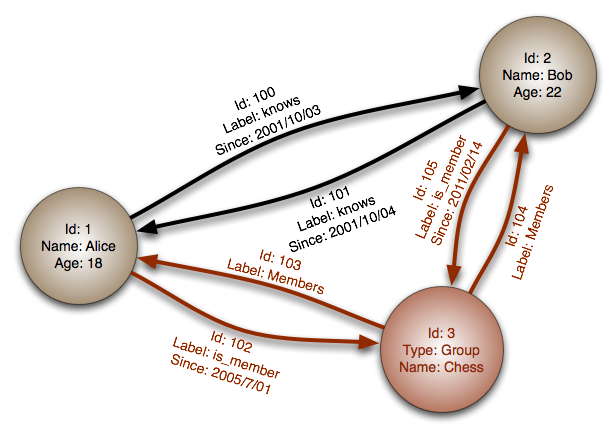
\includegraphics[width=0.7\textwidth]{pics/graph.png}
  \caption{A Graph Database}
 \end{center}
\end{figure}
\\
Owing to these reasons the use of graph database is currently limited. We were motivated to resolve this problem by taking a middle path between graph and relational databases. We wanted to explore the various way to optimize the query execution time as well as the storage of the currently popular relational databases. We also wanted to eliminate all the redundancy in a typical relational database.


\pagebreak
\bibliographystyle{ieeetr}
\bibliography{biblio}
\addcontentsline{toc}{chapter}{Bibliography}
%\addcontentsline{toc}{chapter}{Appendix Paper 1}
%\includepdf[pages={1-9}]{paper1.pdf}
%\addcontentsline{toc}{chapter}{Appendix Paper 2}
%\includepdf[pages={1-6}]{paper2.pdf}
\end{document}